\documentclass[12pt]{article}

%-------------PACKAGES------------- 
\usepackage[margin=1in]{geometry} 
\usepackage{amsmath,amsthm,amssymb}
\usepackage{pgfplots}
\usepackage{float}
\usepackage{braket}
\usepackage{titling}
\usepackage{tikz}
\usepackage{mathtools}
\usepackage{listings}
\usepackage{color}
\usepackage{caption}
\usepackage{subcaption}
\usepackage{algorithm,algpseudocode}

%-------------FORMATTING-------------
\setlength{\droptitle}{-5em} 
\setlength{\parindent}{0pt}
\def\LW{\dimexpr.25\linewidth-.5em} 
 
%--------------COMMANDS--------------
\newcommand{\N}{\mathbb{N}}
\newcommand{\Z}{\mathbb{Z}}
\newcommand{\R}{\mathbb{R}}
\newcommand{\C}{\mathbb{C}}
%\renewcommand{\qedsymbol}{\filledbox}

\DeclarePairedDelimiter \abs{\lvert}{\rvert}%
\DeclarePairedDelimiter \norm{\lVert}{\rVert}%

%------------ENVIRONMENTS------------- 
\newenvironment{theorem}[2][]{\begin{trivlist}
\item[{\bfseries #1}\hskip \labelsep {\bfseries #2.}]}{\end{trivlist}}
\newenvironment{lemma}[2][Lemma]{\begin{trivlist}
\item[\hskip \labelsep {\bfseries #1}\hskip \labelsep {\bfseries #2.}]}{\end{trivlist}}
\newenvironment{exercise}[2][Exercise]{\begin{trivlist}
\item[\hskip \labelsep {\bfseries #1}\hskip \labelsep {\bfseries #2.}]}{\end{trivlist}}
\newenvironment{reflection}[2][Reflection]{\begin{trivlist}
\item[\hskip \labelsep {\bfseries #1}\hskip \labelsep {\bfseries #2.}]}{\end{trivlist}}
\newenvironment{proposition}[2][Proposition]{\begin{trivlist}
\item[\hskip \labelsep {\bfseries #1}\hskip \labelsep {\bfseries #2.}]}{\end{trivlist}}
\newenvironment{corollary}[2][Corollary]{\begin{trivlist}
\item[\hskip \labelsep {\bfseries #1}\hskip \labelsep {\bfseries #2.}]}{\end{trivlist}}
\theoremstyle{remark}
\newtheorem*{remark}{Remark}

%-------------CODE-STYLE------------
\definecolor{dkgreen}{rgb}{0,0.6,0}
\definecolor{gray}{rgb}{0.5,0.5,0.5}
\definecolor{mauve}{rgb}{0.58,0,0.82}
\lstset{frame=tb,
	language=C++,
	aboveskip=3mm,
	belowskip=3mm,
	showstringspaces=false,
	columns=flexible,
	basicstyle={\small\ttfamily},
	numbers=none,
	numberstyle=\tiny\color{gray},
	keywordstyle=\color{blue},
	commentstyle=\color{dkgreen},
	stringstyle=\color{mauve},
	breaklines=true,
	breakatwhitespace=true,
	tabsize=3
}

\lstset{
	morekeywords={end}
}

%------------------------------------ 
%---------START-OF-DOCUMENT----------
%------------------------------------
\begin{document}
 
\title{Program 1}
\author{David Miller \\ 
MAD5403: Foundations of Computational Math I} 
 
\maketitle

\textit{Note: Solutions to analysis problems can be found in sections 3 and 5 labeled according to their respective question on the writeup.}

\section{Executive Summary}
Horner's method is a fast and efficient way of evaluating the polynomial $p_n(x)$. In this program we propose three polynomials in which we numerically approximate via Horner's method and compare it to the "exact" value. Floating point error with respect to single and double precision is also computed and analyzed against a prior error bounds. 

\section{Statement of Problem}

The evaluation of a polynomial $p_n(x)$ is often used in numerics. Thus it is important to have a robust, fast, and efficient algorithm for doing so. Horner's method provides this given the coefficients of the polynomial are known. Horner's method requires $2n$ floating point operations (\textit{flops}), its forward error requires $2n+1$ \textit{flops}, and its running error evaluation requires $4n+1$ \textit{flops}. This leads to a very desired $\mathcal{O}(n)$ time complexity as well $\mathcal{O}(n)$ memory complexity (shown later). In this program we evaluate three polynomials along with their associated errors and "exact: solutions
\begin{itemize}
	\item $p(x) = (x - 2)^9$
	\item $p(x) = (x + 5)^6$
	\item $p(x) = (x - 8)^3$
\end{itemize}
where we use the product form of the polynomial as the "exact" solution. The effect of single and double precision  are also taken into consideration. 

\section{Description of Mathematics}

An error analysis of Horner's rule shows that the computed value of the polynomials satisfies 
\begin{align}
	\tilde{c}_0 = (1 + \theta_1)\alpha_0 + (1 + \theta_3)\alpha_1x + \ldots + (1 + \theta_{2n-1}\alpha_{n-1}x^{n-1} + (1 + \theta_{2n}\alpha_n)x^n
\end{align} 

where $\abs{\theta_k} \leq \gamma_k$ (Higham 2002 Accuracy and Stability of Numerical Algorithms, Second Edition). The pattern on the subscript is odd numbers, i.e., increment of 2, until the last which is even, i.e., last increment is 1. \\
Let 
$$ \tilde{(p_n(x))} = \abs{\alpha_0} + \abs{\alpha_1}x + \ldots + \abs{\alpha_n}x^n. $$

From this we can show that 
\begin{align}
	\frac{\abs{p_n(x) - \tilde{c}_0}}{\abs{p_n(x)}} \leq \gamma_{2n} \frac{\tilde{p}_n(\abs{x})}{\abs{p_n(x)}}
\end{align}

and therefore
$$ \kappa_{rel} = \frac{\tilde{p}(\abs{x})}{\abs{p(x)}} $$
is a relative condition number for perturbations to the coefficients bounded by $\gamma_{2n}$ \\

\textbf{PROBLEM 1.1}
Expanding the numerator of the LHS of (3) we get
\begin{align*}
	\abs{p_n(x) - \tilde{c}_0} & = \big\vert(\alpha_0 + \alpha_1x \ldots + \alpha_{n-1}x^{n-1} + \alpha_nx^n) \\
		 & - ((1 + \theta_1)\alpha_0 + (1 + \theta_3)\alpha_1x + \ldots + (1 + \theta_{2n-1}\alpha_{n-1}x^{n-1} + (1 + \theta_{2n}\alpha_n)x^n))\big\vert \\
		 & = \abs{-\alpha_0\theta_1 - \theta_3\alpha_1 x - \ldots - \theta_{2n-1}\alpha_{n-1}x^{n-1} - \theta_{2n}\alpha_nx^n} \\
		 & \leq \abs{\alpha_0\theta_1} + \abs{\theta_3\alpha_1x} + \ldots + \abs{\theta_{2n-1}\alpha_{n-1}x^{n-1}} + \abs{\theta_{2n}\alpha_nx^n} \\ 
		& \leq \abs{\max\limits_{1 \leq i \leq 2n}(\theta_i)}\abs{\sum\limits_{i=0}^n \alpha_i x^i} \\
		& \leq \abs{\max\limits_{1 \leq i \leq 2n} \theta_i}\sum\limits_{i=0}^n \abs{\alpha_i}\abs{x}^i \\
		& = \abs{\theta_{2n}}\tilde{p}(\abs{x}) \\
		& \leq \gamma_{2n}\tilde{p(\abs{x})}
\end{align*}

Since we have that $\abs{p_n(x) - \tilde{c}_0} \leq \gamma_{2n}\tilde{p}(\abs{x})$ it follows directly that $\frac{\abs{p_n(x) - \tilde{c}_0}}{\abs{p_n(x)}} \leq \gamma_{2n}\frac{\tilde{p}(\abs{x})}{\abs{p_n(x)}}$. From this result we can see that $\frac{\tilde{p}(\abs{x})}{\abs{p(x)}}$ is an amplification factor to the upper bound of relative error $\gamma_k$. We can then conclude that $\kappa_{rel} = \frac{\tilde{p}(\abs{x})}{\abs{p(x)}}$ by definition. \\

\textbf{PROBLEM 1.2} The computed result using Horner's rule and its associated a priori bound, $\abs{\theta_k} \leq \gamma_{2k}$, is backward stable. The computed result $\tilde{c}_0$ is the exact solution to the polynomial 
$$(1 + \theta_1)\alpha_0 + (1 + \theta_3)\alpha_1x + \ldots + (1 + \theta_{2n-1})\alpha_{n-1}x^{n-1} + (1 + \theta_{2n})\alpha_{n}x^n$$ 
where each $\theta_k$ is the perturbation to the coefficients (the data). Since $\theta_k$ is bounded above by $\gamma_k = \frac{k\epsilon_M}{1-k\epsilon_M}$, $k\epsilon_M \approx k\times10^{-7}$ in single precision, and $\approx k\times10^{-16}$ in double precision, we have that $\gamma_k$ is very small and grows at a very slow rate. Therefore we can say that $\tilde{c}_0$ is the exact solution to 
$$(1 + \theta_1)\alpha_0 + (1 + \theta_3)\alpha_1x + \ldots + (1 + \theta_{2n-1})\alpha_{n-1}x^{n-1} + (1 + \theta_{2n})\alpha_{n}x^n$$
for some $\tilde{d}$ in some small neighborhood around our data $d$. \\

\textbf{PROBLEM 1.3} For $p_n(x)$ to be perfectly conditioned with respect to perturbations to the coefficients of the monomial form we must have that $\frac{\tilde{p}(\abs{x})}{\abs{p(x)}} = 1.$ If we expand this fraction we can see when this happens:
\begin{align*}
	\frac{\tilde{p}(\abs{x})}{\abs{p(x)}} & = \frac{{\abs{\alpha_0} + \abs{\alpha_1}\abs{x} + \ldots \abs{\alpha_{n-1}}\abs{x}^{n-1} + \abs{\alpha_n}\abs{x}^n}}{\abs{\alpha_0 + \alpha_1x + \ldots \alpha_{n-1}x^{n-1} + \alpha_nx^n}} \\
	& = 
	\begin{cases}
		\frac{\abs{\alpha_0} + \abs{\alpha_1}x + \ldots + \abs{\alpha_{n-1}x^{n-1} + \abs{\alpha_n}x^n}}{\abs{\alpha_0 + \alpha_1x + \ldots \alpha_{n-1}x^{n-1} + \alpha_nx^n}} & x > 0 \\
		\frac{{\abs{\alpha_0} + \abs{\alpha_1}\abs{x} + \ldots \abs{\alpha_{n-1}}\abs{x}^{n-1} + \abs{\alpha_n}\abs{x}^n}}{\abs{\alpha_0 - \alpha_1\abs{x} + \alpha_2x^2 - \alpha_3\abs{x}^3 + \ldots}} & x < 0 \\
		\hspace{2.5cm} 1 & x = 0
	\end{cases} \\
	& = 
	\begin{cases}
	1 & x > 0, sign(\alpha_i) = sign(\alpha_j) \, \forall i,j \\
	1 & x < 0, sign(\alpha_{i}) = sign(\alpha_{i=2}), \\ & sign(\alpha_i) \neq sign(\alpha_{i+1}) \, \forall i \\
	1 & x =0
	\end{cases}
\end{align*}
Therefore if we evaluate $p_n(x)$ for some $x \in \mathbb{R}^+$ we must have that all the coefficients have the same sign for perfectly conditioned. However, if we evaluate $p_n(x)$ for some $x \in \mathbb{R}^-$ then we must have coefficients with alternating signs for perfectly conditioned. The case when we evaluate $p_n(x)$ at $x = 0$ is perfectly conditioned. \\

\textbf{PROBLEM 1.4} Now let's assume that our polynomial is not perfectly conditioned. We can then model the behavior of our conditioning number as it approaches some root $x_0$ for the polynomial $p(x)$:

\begin{align*}
	\lim_{x \rightarrow x_0}\kappa & = \lim\limits_{x \rightarrow x_0} \frac{\tilde{p}(\abs{x})}{\abs{(p(x)}} \\
	& = \lim\limits_{x \rightarrow x_0} \frac{\abs{\alpha_0} + \abs{\alpha_1}\abs{x_0} + \ldots + \abs{\alpha_{n-1}}\abs{x_0}^{n-1} + \abs{\alpha_n}\abs{x_0}^n}{\abs{\alpha_0 + \alpha_1x_0 + \ldots + \alpha_{n-1}x_0^{n-1} + \alpha_nx_0^n}}
\end{align*}

The last expression will blow up if $x_0$ is not a root for $\tilde{p}(\abs{x})$. Therefore I would expect $p_n(x)$ to be relatively sensitive when we are near some point $x_0$ such that $p(x_0) = 0$ and $\tilde{p}(\abs{x}) \neq 0$ since the conditioning number $\kappa$ will be some large number. \\

\textbf{{PROBLEM 3}} Forward error provides a decent bound, but a much tighter bound for Horner's method can be computed if we calculate some error at each step, we will define this as the running error. The computed value on step $i$ of Horner's rule satisfies
$$ (1 + \epsilon_i)\hat{c}_i = x\hat{c}_{i+1}(1 + \delta_i) + \alpha_i, \quad \abs{\delta_i} \leq u, \abs{\epsilon_i} \leq u $$

If we let $\hat{c}_i = c_i + e_i, e_n = 0$ and $c_i$ the exact value of the parameter in Horner's rule evaluated in exact arithmetic. Working off of this we can derive the forward error at each step:
\begin{align*}
	\hat{c}_i + \epsilon_i\hat{c}_i & = x\hat{c}_{i+1} + \delta_ix\hat{c}_{i+1} + \alpha_i \\
	\Rightarrow \, \hat{c}_i + e_i + \epsilon_i\hat{c}_i & = x(\hat{c}_{i+1} + e_{i+1}) + \delta_ix(c_{i+1} + e_{i+1}) + \alpha_i \\
	& = x\hat{c}_{i+1} + xe_{i+1} + \delta_ixc_{i+1} + \delta_ixe_{i+1} + \alpha_i \\
	\Rightarrow \, e_i + \epsilon_i\hat{c}_i & = xe_{i+1} + \delta_ixc_{i+1} + \delta_ixe_{i+1} \\ 
	e_i & = xe_{i+1} - \epsilon_i\hat{c}_i + \delta_ix({c}_{i+1} + e_{i+1}) \\
	\Rightarrow \, e_i & = xe_{i+1} - \epsilon_i\hat{c}_i + \delta_ix\hat{c}_{i+1}
\end{align*}

Now that we have what the running error is for each step of Horner's rule we would like to find an upper bound on this. Given
$$ \beta_i = \abs{x}\beta_{i+1} + \abs{x}\abs{\hat{c}_{i+1}} + \abs{\hat{c}_i} $$
and $\beta_n = e_n = 0$ we can compute $B_{n-1}$ along with $e_{n-1}$
\begin{align*}
	\beta_{n-1} & = \abs{x}\beta_{n} + \abs{x}\abs{\hat{c}_{n}} + \abs{\hat{c}_{n-1}} = \abs{x}\abs{\hat{c}_{n}} + \abs{\hat{c}_{n-1}} \\
	e_{n-1} & = xe_n - \epsilon_{n-1}\hat{c}_{n-1} + \delta_{n-1}x\hat{c}_n = \delta_{n-1}x\hat{c}_n - \epsilon_{n-1}\hat{c}_{n-1}
\end{align*}

Its easy to see from the above that $\abs{e_n} \leq u\beta_n$ where $u$ is machine epsilon. It also follows from continuing this iteration that this inequality will hold for all $i = 0,1,\ldots,n$.

\section{Description of the Algorithm and Implementation}
Horner's method evaluates $p_n(x)$ by building the polynomial inside out. Inside the \texttt{for loop} is has 2 \textit{flops} for $n$ iterations, therefore the time complexity is $\mathcal{O}(n)$. The coefficients must be stored in some data structure as well as some variable to store the value computed at each step, therefore the memory complexity is $\mathcal{O}(n)$. \\ \\
\textbf{Input:} Point $x$, Coefficients $\{\alpha_0,\ldots,\alpha_n\}$ \\
\textbf{Output:} Evaluation of polynomial $p(x	)$
\vspace{-0.3cm}
\begin{algorithm}[H]
	\caption{Horner's Method}
	\begin{algorithmic}[1]
		\State{$q_n(x)$ $\leftarrow$ $\alpha_n$}	
		\For{$i = n-1:-1:0$}
		\State{$q_i(x)$ $\leftarrow$ $xq_{i+1}(x)$ + $\alpha_i$}
		\EndFor
		\State{$p(x) \leftarrow q_0(x)$}
		\State{\textbf{return} $p(x)$}	 
	\end{algorithmic}
\end{algorithm}

The forward error computation is similar to Horner's method. The only difference is taking the absolute value of $x$  and $\alpha_i$ at each iteration. There is one extra flop and that is at the end when multiplying by $\gamma_{2n}$. Therefore we have that the time and memory complexity is $\mathcal{O}(n)$. \\ \\
\textbf{Input:} Point $x$, Coefficients $\{\alpha_0,\ldots,\alpha_n\}$ \\
\textbf{Output:} Forward Error $\epsilon_F$
\vspace{-0.3cm}
\begin{algorithm}[H]
	\caption{Forward Error}
	\begin{algorithmic}[1]
		\State{$\tilde{p}_n(x)$ $\leftarrow$ $\alpha_n$}	
		\For{$i = n-1:-1:0$}
		\State{$\tilde{p}_i(x)$ $\leftarrow$ $\abs{x}\tilde{p}_{i+1}(x)$ + $\abs{\alpha_i}$}
		\EndFor
		\State{$\epsilon \leftarrow \gamma_{2n} \star \tilde{p}_0(x)$}
		\State{\textbf{return} $\epsilon_F$}	 
	\end{algorithmic}
\end{algorithm}
\vspace{-0.65cm}
{\scriptsize Where we define $\gamma_{k} = k\epsilon_M/(1 - k\epsilon_M)$ for some machine epsilon $\epsilon_M$.} \\

The running error calculation (not including Horner's method in the calculation) performs 4 \textit{flops} per iteration. It performs 3 before before an evaluation of Horner's method is done then another one when we add the result to the running error. Therefore the time complexity of running error is $\mathcal{O}(n)$. Since we have to store the coefficients and a variable we have that the memory complexity is $\mathcal{O}(n)$. \\ \\
\textbf{Input:} Point $x$, Coefficients $\{\alpha_0,\ldots,\alpha_n\}$ \\
\textbf{Output:} Running Error $\epsilon_R$
\vspace{-0.3cm}
\begin{algorithm}[H]
	\caption{Running Error}
	\begin{algorithmic}[1]
		\State{$q_n(x)$ $\leftarrow$ $\alpha_n$}
		\State{$\epsilon_n$ $\leftarrow$ 0}	
		\For{$i = n-1:-1:0$}
		\State{$\epsilon_i$ $\leftarrow$ $\abs{x}\abs{e_{i+1}}$ + $\abs{x}\abs{q_{i+1}(x)}$}
		\State{$q_i(x)$ $\leftarrow$ $xq_{i+1}(x)$ + $\alpha_i$}
		\State{$\epsilon_i$ $\leftarrow$ $\epsilon_{i+1} + q_i(x)$}
		\EndFor
		\State{$\epsilon_R \leftarrow \epsilon_M\epsilon_0$}
		\State{\textbf{return} $\epsilon_R$}
	\end{algorithmic}
\end{algorithm}
\vspace{-0.65cm}
{\scriptsize Where we define $\epsilon_M$ as machine epsilon for the specified precision.} 

\section{Description of the Experiment Design and Results}

The execution of the code can be summarized as follows
\begin{itemize}
	\item The user specifies what polynomial and precision to use; these computations are done in C++.
	\subitem Single precision: \texttt{g++ -std=c++11 -DSINGLE=1 main.cpp}
	\subitem Double precision: \texttt{g++ -std=c++11 -DDOUBLE=1 main.cpp}
	\item The computations are written to some file
	\item The data is read and graphed; this is done with Python.
\end{itemize}	
The \texttt{main function} simply iterates over some domain using a $\Delta x$ to move forward. Within these iterations our three main algorithms are called and their results are written to a specified file. The logic of the program is simple and easy to understand.

The three polynomials that were chosen are 
$$ p(x) = (x-8)^3, \quad p(x) = (x+5)^6, \quad p(x) = (x-2)^9 $$.
We choose these polynomials for several reasons:
\begin{enumerate}
	\item Investigate how the degree of the polynomial affects the accuracy and error of Horner's method,
	\item Investigate how the magnitude and sign of the root affect the accuracy and errors of Horner's method
	\item Investigate the sensitivity (conditioning) of Horner's method near the roots.
\end{enumerate}
From figures (1) - (3) we can see that the magnitude of our errors are relative to both the degree of the polynomial and the magnitude of our root. Figure (3) has much tighter bounds than that of figure (1). Another way to verify this is to notice that our forward error bound magnitude increases as $x$ increases in figure (1) and increases as $x$ decreases in figure (2) (this is because we are in a negative domain). \\

\textbf{PROBLEM 2.3} The fact that we used single precision when calculating the a priori bound is of importance. This is because $\epsilon_M \approx 10^{-7}$ in single precision while $\epsilon_M \approx 10^{-16}$ in double precision. Thus double precision bounds will be many magnitudes smaller than that of single precision resulting in forward and error running bounds using double precision being too strict for Horner's method in single precision. This is clearly shown in figure (4).
\section{Conclusions}

From our results and analysis we can see that Horner's method evaluates $p_n(x)$ in $\mathcal{O}(n)$ time complexity and $\mathcal{O}(n)$ memory complexity with errors proportional to $n$ and the precision used. Our forward error bounds provide a lenient bound while our running error bound provides a bound approximately 20 times tighter than forward error. Horner's method, when evaluated in the same precision as the error, falls within the error bounds illustrating that it is a very accurate algorithm. We also verified that computing the "exact" evaluation using the product form in single precision yields almost identical results to that of double precision. Lastly we illustrated that Horner's method has varying sensitivity with respect to $x$. We confirmed that higher conditioning numbers incur high sensitivity to perturbations in our data. If we want a polynomial with a low conditioning number than we should try to minimize the degree and magnitude of the root.

\section{Figures} 

\begin{figure}
	\vspace{-2.2cm}
	\begin{center}
		{\LARGE $p(x) = (x-2)^9$}
	\end{center}
	\parbox{\LW}{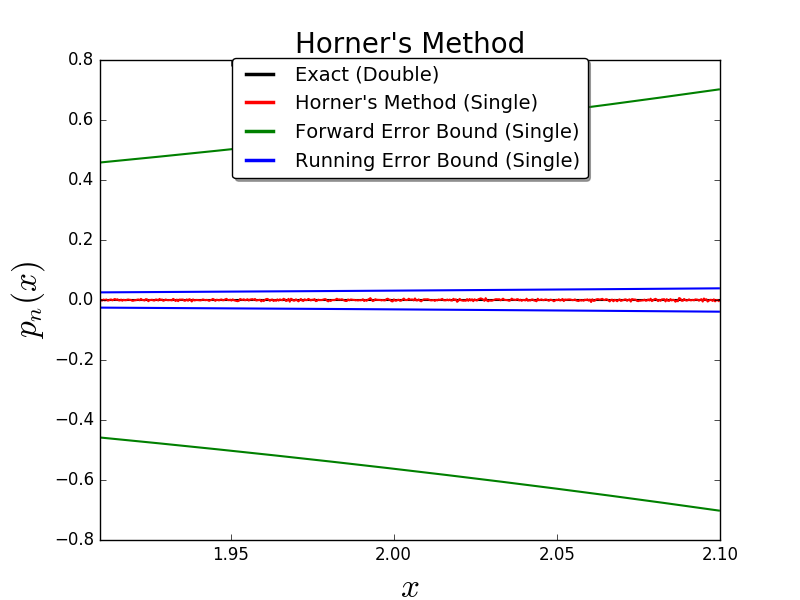
\includegraphics[width=11cm]{Single1.png}}\hfill%
	\parbox{\LW}{\subcaption{Global figure showing the "exact" polynomial evaluation, Horner's method, forward error bounds, and running error bounds on the entire domain [1.91,2.1].}}\hfill \\
	\parbox{\LW}{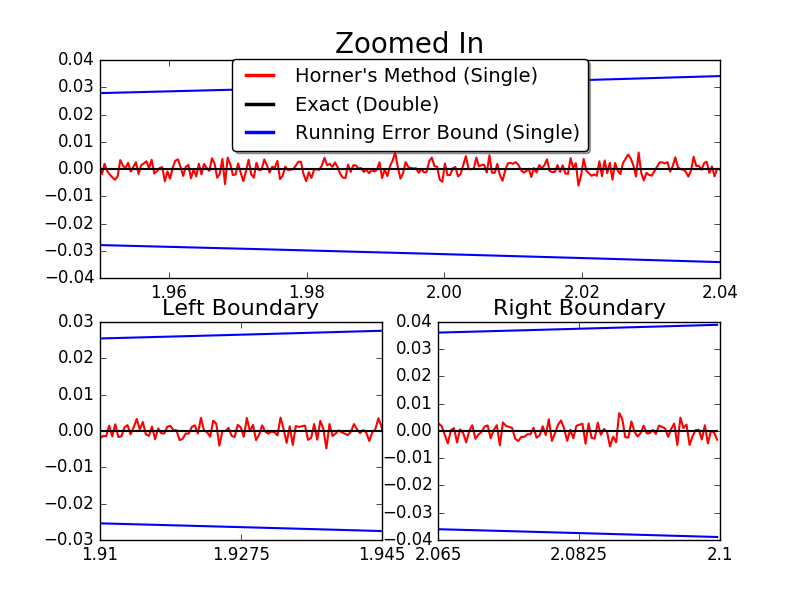
\includegraphics[width=11cm]{Single2.png}}\hfill%
	\parbox{\LW}{\subcaption{Local figure showing the "exact" polynomial evaluation, Horner's method, and running error bounds on the left boundary, right boundary, and middle.}} \\	\parbox{\LW}{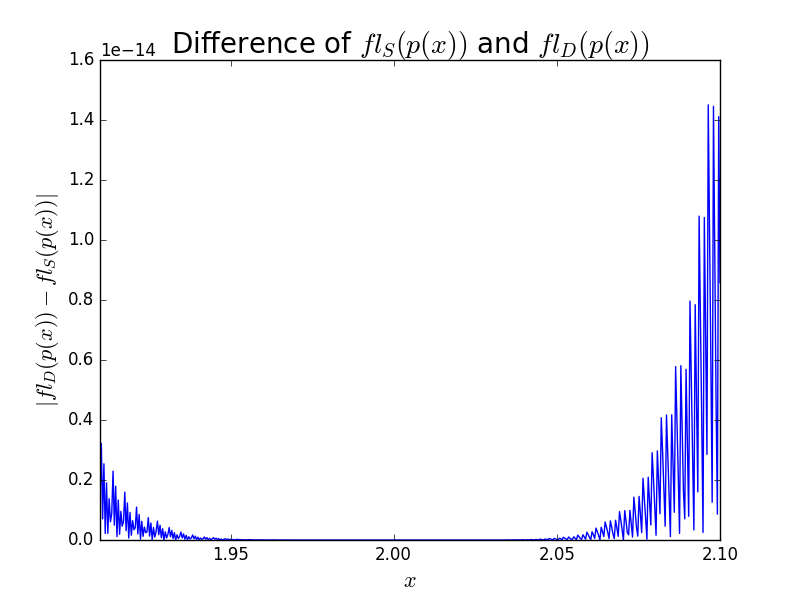
\includegraphics[width=11cm]{dif1.png}}\hfill%
	\parbox{\LW}{\subcaption{The absolute difference between "exact" computations done in single and double precision.}}
	\caption{Numerical results for $p(x) = (x-2)^9$.}
\end{figure}  

\begin{figure}
	\vspace{-2.2cm}
	\begin{center}
		{\LARGE $p(x) = (x+5)^6$}
	\end{center}
	\parbox{\LW}{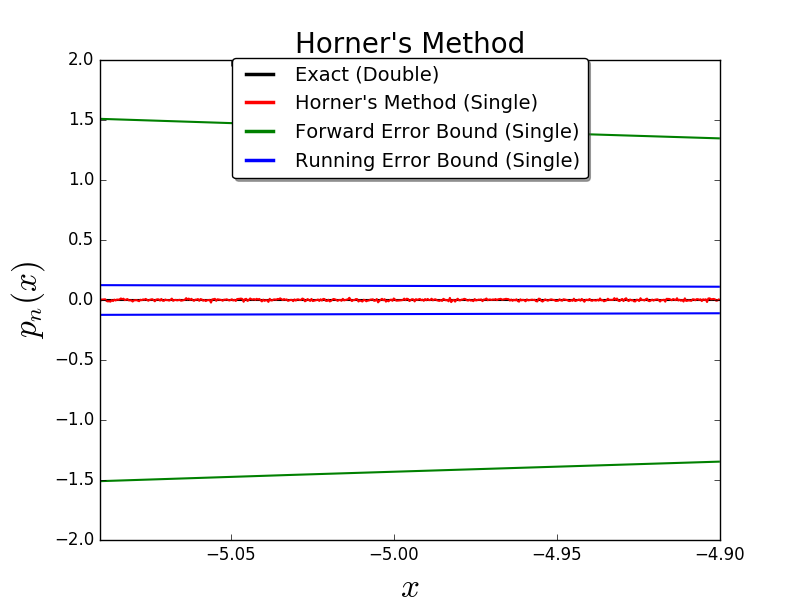
\includegraphics[width=11cm]{Single3.png}}\hfill%
	\parbox{\LW}{\subcaption{Global figure showing the "exact" polynomial evaluation, Horner's method, forward error bounds, and running error bounds on the entire domain [-5.09,-4.9].}}\hfill \\
	\parbox{\LW}{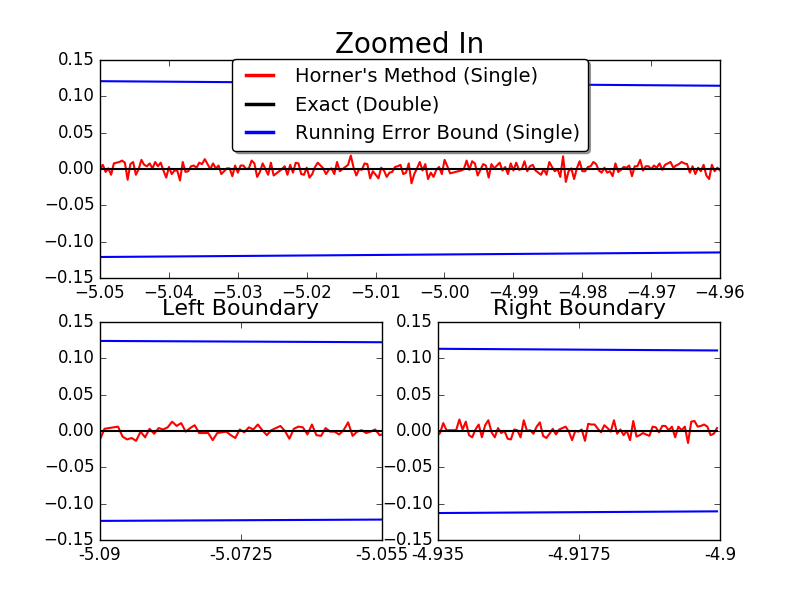
\includegraphics[width=11cm]{Single4.png}}\hfill%
	\parbox{\LW}{\subcaption{Local figure showing the "exact" polynomial evaluation, Horner's method, and running error bounds on the left boundary, right boundary, and middle.}} \\	\parbox{\LW}{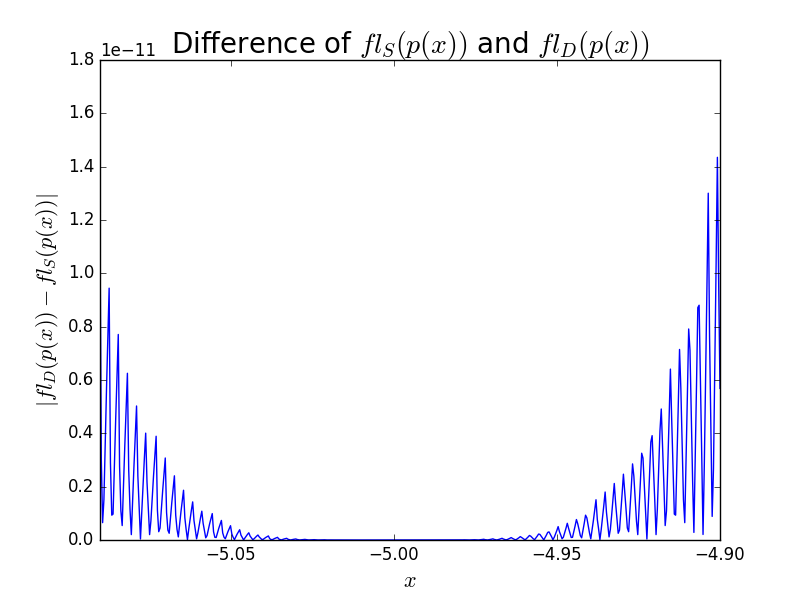
\includegraphics[width=11cm]{dif2.png}}\hfill%
	\parbox{\LW}{\subcaption{The absolute difference between "exact" computations done in single and double precision.}}
	\caption{Numerical results for $p(x) = (x+5)^6$.}
\end{figure}

\begin{figure}
	\vspace{-2.2cm}
	\begin{center}
		{\LARGE $p(x) = (x-8)^3$}
	\end{center}
	\parbox{\LW}{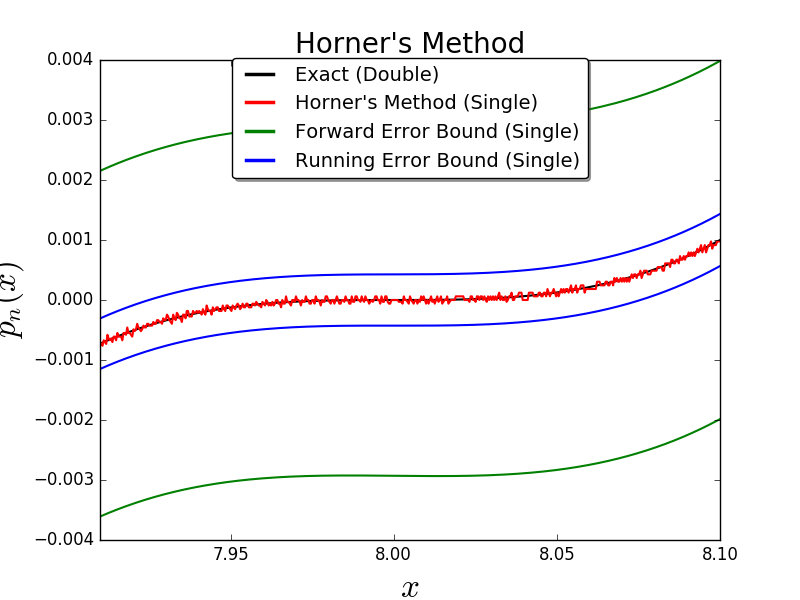
\includegraphics[width=11cm]{Single5.png}}\hfill%
	\parbox{\LW}{\subcaption{Global figure showing the "exact" polynomial evaluation, Horner's method, forward error bounds, and running error bounds on the entire domain [7.91,8.1].}}\hfill \\
	\parbox{\LW}{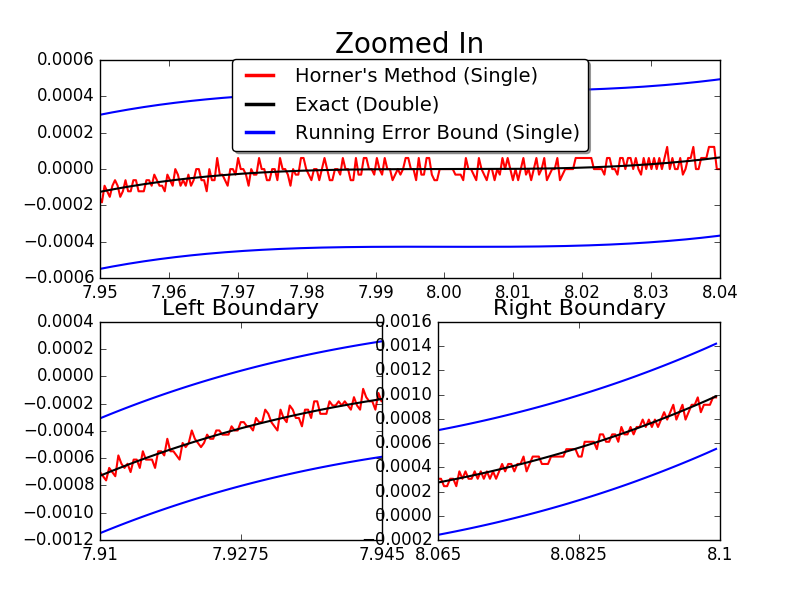
\includegraphics[width=11cm]{Single6.png}}\hfill%
	\parbox{\LW}{\subcaption{Local figure showing the "exact" polynomial evaluation, Horner's method, and running error bounds on the left boundary, right boundary, and middle.}} \\	\parbox{\LW}{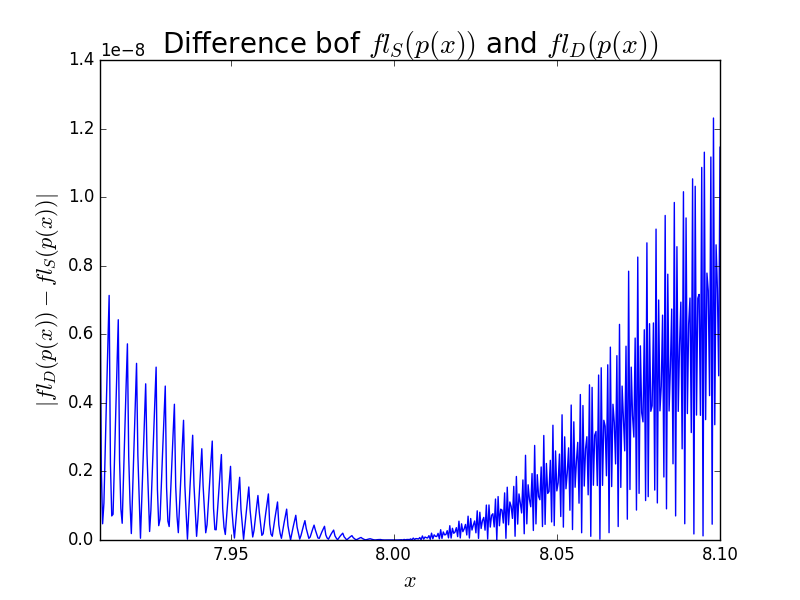
\includegraphics[width=11cm]{dif3.png}}\hfill%
	\parbox{\LW}{\subcaption{The absolute difference between "exact" computations done in single and double precision.}}
	\caption{Numerical results for $p(x) = (x-8)^3$.}
\end{figure}  

\newpage

\begin{figure}[H]
	\centering
	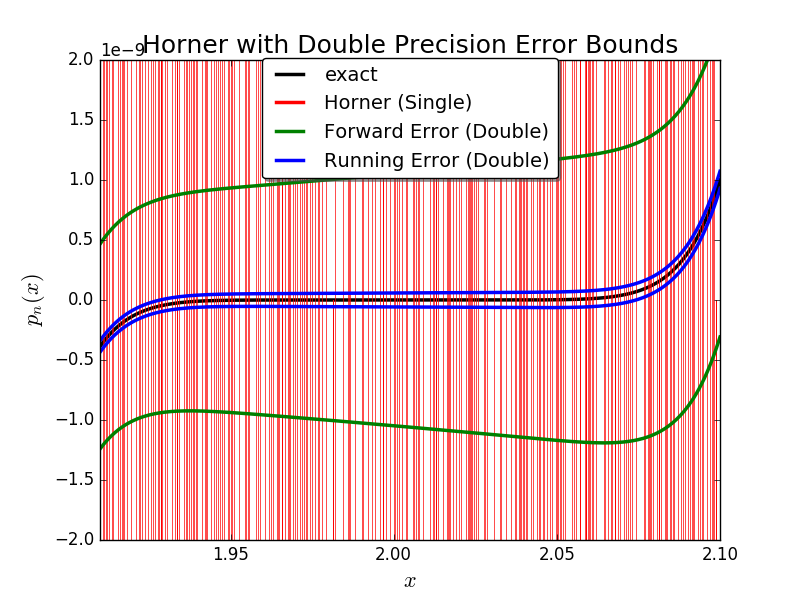
\includegraphics[width = 15cm]{singleHornerdoubleErro.png}
	\caption{Horner's method calculated using single precision and error bounds using double precision. This does not yield useful results since Horner's method returns values outside of the bounds.}
\end{figure}

\section{References}

I used a suggested format for my code provided at \\

https://stackoverflow.com/questions/14511910/switching-between-float-and-double-precision-at-compile-time

\end{document}
